\section{Introduction}

The key to solving absolute value 
\myEmph{equations} was to think about \gap{distance}.

\begin{tcolorbox}[width=4in, center, colback=white,]
    $|x| = 3$
    \tcblower
    \begin{center}
        \begin{tcolorbox}[center,colback=white,boxrule=0.5pt,]
            \small The distance of $x$ from the origin is \myEmph{equal to} $3$.
        \end{tcolorbox}
        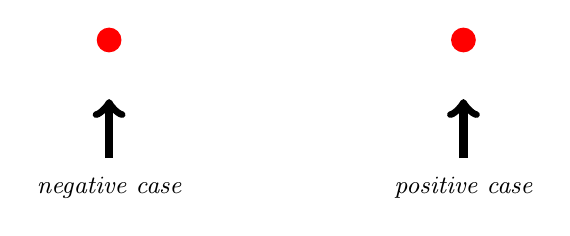
\begin{tikzpicture}[scale=0.75]
            \myDrawNumberlineCircle{0}{white}
            \whenTEACHER{
                % \draw [->,line width=3pt,red] (-3,-2) -- (-3,-1);
                \draw[red,line width=2.5pt,fill=red] (-3,0) circle (0.15 cm);
                %
                % \draw [->,line width=3pt,red] (3,-2) -- (3,-1);
                \draw[red,line width=2.5pt,fill=red] (3,0) circle (0.15 cm);
                }
                \draw[->, black, line width=3pt] (-3,-2) -- (-3,-1);
                \node[] at (-3,-2.5) {\itshape\small negative case};
                \draw[->, black, line width=3pt] (3,-2)  -- (3,-1);
                \node[] at (3,-2.5) {\itshape\small positive case};
                \myDrawNumberline{5}
        \end{tikzpicture}\\
        \whenSTUDENT{\vspace{3\onelineskip}}
        %
        \whenTEACHER{
            {
                $x = -3$
            }
            \hfil
            {
                $x = 3$
            }
        }
    \end{center}
\end{tcolorbox}

Similarly,
the key to solving absolute value
\myEmph{inequalities} is to think about \gap{distance}.

